\chapter{Analysis and Implementation}

In this chapter we analyze the algorithm used to process EBSD data and explain how to implement it effectively for GPUs. We use the CUDA platform, which is currently the most popular technology for general purpose computing on graphics cards.

\todo{CUDA summary?}

The input for the algorithm consists of one reference and many deformed backscatter patterns which are captured in greyscale images. There may be up to tens of thousands of them. In general, the format of the pictures is not important, as long as it is possible to load them from disk quickly. For example, our testing data consists of 15000 images saved in TIFF format without any compression. Each picture has resolution of approximately $900 \times 900$ pixels and each pixel is represented by a 16 bit unsigned integer --- the higher the integer, the higher is the luminosity of the pixel.

The result of the algorithm is a list of two--dimensional vectors that we write to the standard output.

There are further parameters to the algorithm explained in the \cref{chap1}. \Cref {params} summarizes them along with the range of values that we consider.

\begin{table}[]
	\centering
	\begin{tabular}{@{}lll@{}}
		\toprule
		Parameter                  & Label            &    Value range  \\ \midrule
		Size of input pattern      & $W_p \times H_p$ & $640 \times 480$\footnotemark  -- $1400 \times 1000$ \footnotemark  \\
		Number of subregions       & $S$              &               10 -- 100 \\
		Size of a subregion        & $W_r \times H_r$ & $50 \times 50$ -- $250 \times 250$ \\
		Diameter of a neighborhood & $F$              &                3,5,7,9 \\ \bottomrule
	\end{tabular}
	\caption{Summary of algorithm parameters with example values that show their order of magnitude.}
	\label{params}
\end{table}
\footnotetext[1]{\url{https://www.edax.com/products/ebsd/digiview-ebsd-camera}}
\footnotetext{\url{https://www.eden-instruments.com/en/download/hikari-ebsd-camera-series/}}

\if{false}
From a high--level point of view, the algorithm first loads reference pattern from disk. Then it goes through a list of file names of deformed images and does 3 steps with each:
\begin{enumerate}
	\item Load a deformed pattern from disk.
	\item Compare the deformed and reference patterns.
	\item Write the resulting offsets to standard output.
\end{enumerate}
While the steps 1 and 3 have to be done by the CPU, the second step is suitable for execution on a GPU.

As explained in the previous chapter, the comparison of two patterns is done by cross--correlating several subregions of the images and then finding the offset for which the correlation is maximal. Location, size and number of the subregions is a parameter for the algorithm; we expect that there will be tens of subregions with size in the order of $100 \times 100$ pixels. All the subregions in all the images are processed independently from each other, providing a great opportunity to utilize data parallelism.



The processing of each subregion is done in several steps:
\begin{enumerate}
	\item Normalize the pixels of the subregion --- compute its mean and subtract it from each pixel
	\item Cross--correlate deformed region with the reference one
	\item Find the position of the maximum (argmax) in the cross--correlation
	\item Use the neighborhood of the maximum to ``interpolate'' and find the most probable offset of the subregion with subpixel accuracy
\end{enumerate}

These steps can be executed in parallel for all the subregions of one pattern. So every time we start a kernel, it executes the step for all the subregions of the pattern. We can go even further and process the subregions of several patterns, i.e., a batch of patterns, at the same time. This approach can help to increase the GPU utilization, especially when there are only few subregions in each pattern. In the rest of the chapter, we mostly describe the algorithm for one pattern only, because it is not very hard to expand it for batches of patterns.

\fi



\section{Cross--correlation}
We start by analyzing the core of the algorithm --- cross--correlation, which is also the most computationally expensive part. The input for cross--correlation are two images, in our case it is a deformed and a reference subregion. More precisely, there are several pairs of subregions, but since they are completely independent, we explain the algorithm for one pair only. With respect to the definition in \cref{cross-corr-def}, we cross--correlate the reference with deformed subregion, i.e. $reference \star deformed$, not the other way around. Also, both subregions are of the same size, which simplifies some aspects of the algorithm.

\subsection{Related work}

Since cross--correlation is quite a common operation in image processing, various researchers implemented it on GPUs. For example, Liu, Zou and Luo implemented the cross--correlation for CUDA 3.1 using the cuFFT library in 2011 \cite{liu2011gpu}. Lewis explained how to optimize computation of normalized cross--correlation denominator \cite{lewisfast} and Gangodkar et al. implemented it for GPU \cite{gandokar2012fastNCCGPU}. It is also used as part of various image processing algorithms, for example Idzenga, Gaburov, Vermin, Menssen and De Korte used a GPU implementation of normalized cross--correlation for ultrasound images analysis \cite{Idzenga2014Ultrasonics}.

There are also libraries that can leverage GPUs to compute cross--correlation. Matlab has a function called \texttt{xcorr2} that can be GPU--accelerated \cite{MATLAB:2018}.  npp

convolution?


 We first describe a naive algorithm designed directly from the definition. Then we explain another implementation that uses discrete Fourier transform. The reason why we implement two versions is that although the Fourier transform based implementation has better asymptotic complexity, the subregions may not be big enough to reflect it.



A serial algorithm for cross--correlation is shown in algorithm \ref{crossAlgo}. It is directly based on the definition. It iterates over all possible shifts between the images (subregions), i.e. $\forall [shiftX, shiftY] \in (-W_s, W_s) \times (-H_s, H_s)$. Shifts that are further from zero than width (height) of the picture are always zero, since the second subregion is shifted so far that they do not overlap at all. For each of the shifts $[shiftX, shiftY]$, we sum over the products of pixels that overlap when we shift the deformed subregion by shiftX pixels horizontally and by shiftY vertically.



\begin{algorithm}
	\caption{Serial algorithm that computes cross--correlation.}
	\label{crossAlgo}
	\KwIn{reference: an array of pixels of a reference subregion \newline
		deformed: an array of pixels of a deformed subregion \newline
		$W_s, H_s$: size of both subregions}
	\KwOut{result: cross--correlation between reference and deformed subregions}
	\vspace{5px}
	
	\For{$\text{shiftX} \in (-W_s, W_s)$}{
		\For{$\text{shiftY} \in (-H_s, H_s)$}{
			sum = 0\;
			\For{$x \in [0, W_s)$}{
				\For{$y \in [0, H_s)$}{
					shiftedX = x + shiftX\;
					shiftedY = y + shiftY\;
					\If{$\text{shiftedX} \in [0,W_s]$ \textbf{and} $\text{shiftedY} \in [0,H_s]$}{
						sum += reference[x,y] * \newline deformed[shiftedX, shiftedY]\;
					}
				}
			}
			result[shiftX, shiftY] = sum\;
		}
	}
\end{algorithm}

\begin{algorithm}
	\caption{Pseudocode of CUDA kernel that computes cross--correlation.}
	\label{crossKernel}
	
	shiftX = threadId.x\;
	shiftY = threadId.y\;
	intervalX = $\text{shiftX} < 0$ ? $[-\text{shiftX}, W_s]$ : $[0, W_s - \text{shiftX}]$\;
	intervalY = $\text{shiftY} < 0$ ? $[-\text{shiftY}, H_s]$ : $[0, H_s - \text{shiftY}]$\;
	
	sum = 0\;
	\For{$x \in [0, \text{intervalX})$}{
		\For{$y \in [0, \text{intervalY})$}{
			shiftedX = x + shiftX\;
			shiftedY = y + shiftY\;
			sum += reference[x,y] * deformed[shiftedX, shiftedY]\;
		}
	}
	result[shiftX, shiftY] = sum\;
	
\end{algorithm}

The inner two loops of the algorithm iterate through all pixels of the reference image. However that is not necessary for all shifts, since for most of them only smaller parts of the images overlap (the only shift that requires iteration through all points is $[0,0]$). The if statement then filters out the pixels that do not overlap for specific shift. For performance reasons, we can get rid of the if statement, if we rewrite the two inner loops to always stay within the boundaries of the images.

We will reason only about $shiftX$, since the same argumentation applies to $shiftY$. So we are asking the following question: for which $x \in [0, W_s)$, it holds that $(x + shiftX) \in [0, W_s)$, if $shiftX \in (-W_s, W_s)$? We divide $shiftX$ into negative and nonnegative values:
\begin{itemize}
	\item $\forall shiftX \in (-W_s, 0): (x + shiftX) \in [0, W_s) \iff x \in [-shiftX, W_s]$
	\item $\forall shiftX \in [0, W_s): (x + shiftX) \in [0, W_s) \iff x \in [0, W_s - shiftX]$
\end{itemize}
This gives us an interval through which we iterate $x$ in the inner loops for each \IT{shiftX}. Similar modification applies for the y loop based on \IT{shiftY} as well.

The modified algorithm written as a CUDA kernel is listed in algorithm~\ref{crossKernel}. We implemented the algorithm for CUDA by parallelizing over the outer two loops. That means each thread computes one shift and thus one value of the result. It uses two--dimensional blocks, so we can just use the two indices as \IT{shiftX} and \IT{shiftY}. For computing more subregions at a time, we simply use more threads.



\subsection{The cuFFT library}
We now move on to explain our implementation of the cross--correlation computation using the Fourier transform. We use the cuFFT\footnote{\url{https://docs.nvidia.com/cuda/cufft/index.html}} library for CUDA to compute the discrete Fourier transform and its inverse. It is a highly optimized implementation of the \emph{Fast Fourier algorithm}, which computes the Fourier transform in time $\mathcal{O}(n \log n)$. It also supports batched transformations (i.e. several unrelated transformations can be done by calling single library function), which is very important for our implementation, since we do many transformations of rather small images at once. In this section, we explain the implementation for one subregion only, since it is trivial to expand it for more subregions.

There are two functions in the cuFFT library that are essential for us \texttt{R2C} and \texttt{C2R}, which compute the discrete Fourier transform and its inverse, respectively. \texttt{R2C} takes an array of real numbers and computes their discrete Fourier transform, outputting an array of complex numbers. A complex number is represented as a pair of floats/doubles. The \texttt{C2R} function takes an array of complex numbers, computes their inverse Fourier transform and outputs an array of real numbers.

Both of the functions use an important property of Fourier transform: A series $x$ of $N \in \mathbb{N}$ numbers is real-valued if and only if the Fourier transform of $x$ denoted as $X$ satisfies the Hermitian symmetry, e.g. $X_k = X_{N-k}^\star$. So it is enough to store just half of the transformed array, since the second half can be trivially computed. cuFFT does just that. Analogous theorem applies to two--dimensional Fourier transform as well, so cuFFT operates on roughly half of the elements, namely on the elements with index from the following set: $\{0,1,\cdots, \floor{W/2} + 1\} \times \{0, 1, \cdots, H\}$, where $H$ is number of rows and $W$ is number of columns of the input matrix.

It also makes it possible to store the Fourier transform in roughly the same array as the input and thus perform in--place transforms. The output consists of complex numbers, which are represented by two real numbers, i.e., one element takes twice as much bytes. But at the same time, we only need $W/2 + 1$ columns (we can remove the floor operator, because $W$ is always even in our context as we double the size of a subregion with zero padding). The result is that we save the input in a real matrix with size $(W+2) \times H$, with the two extra columns unused. That is the same amount of space that we need for the transformed complex matrix with size $W/2 + 1 \times H$.

\subsection{Using cuFFT to compute cross--correlation}

\Cref{fft-impl} shows the process with illustration of used buffers. Recall that we cross--correlate a deformed subregion with a reference, both with size $W_s \times H_s$. The preparation kernel extracts the data from the input pattern and outputs it directly into a zero--padded buffer with size $2W_s \times 2H_s$. Then, we use the \texttt{R2C} function from the cuFFT library to compute Fourier transform of the padded deformed subregion. The result is another buffer with size $(W_s + 1) \times 2H$ of complex numbers, which is the same as $(2W_s+2) \times 2H_s$ of real numbers.

\begin{figure}
	\centering
	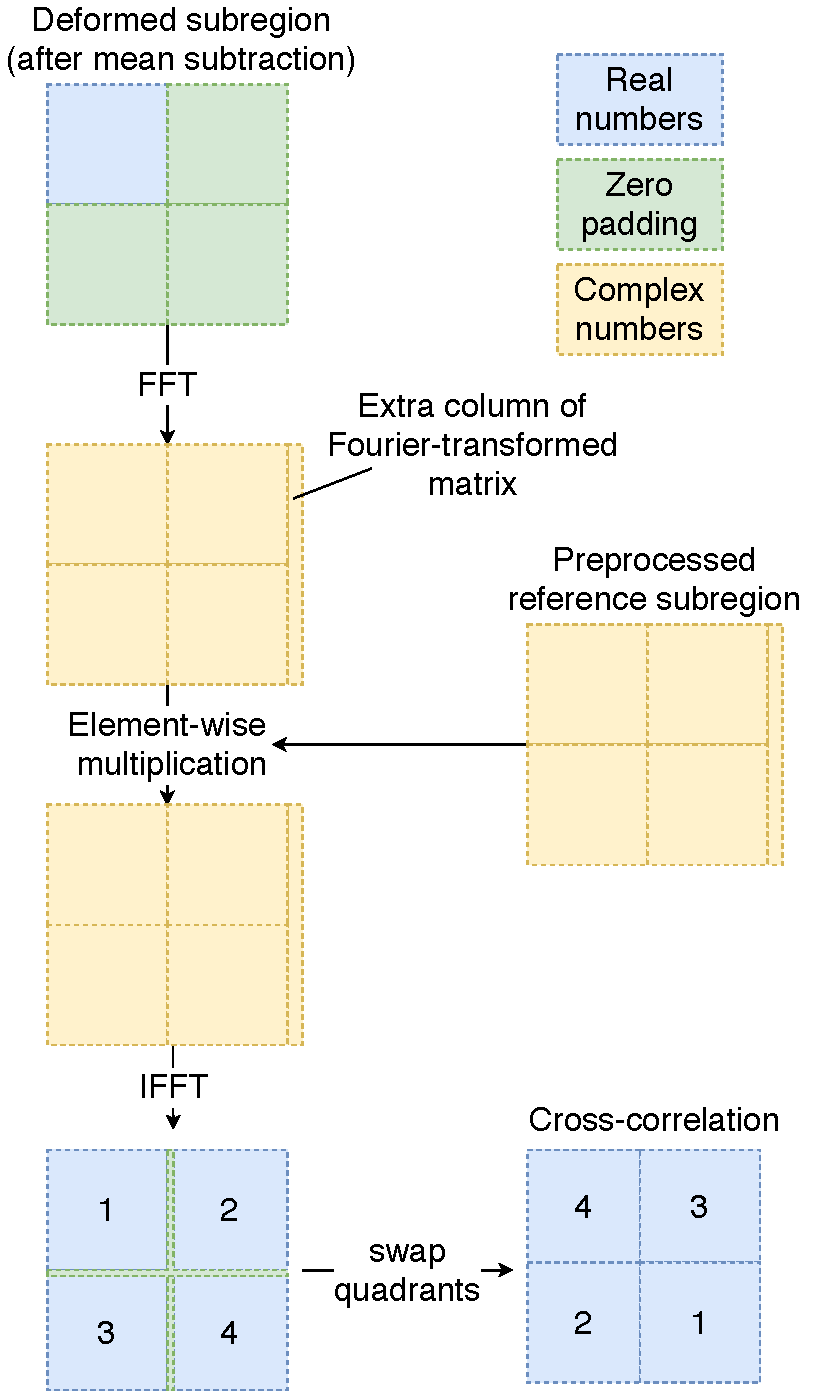
\includegraphics[width=0.7\textwidth]{img/fft-impl}
	\caption{The process of computing cross--correlation using the discrete Fourier transform.}
	\label{fft-impl}
\end{figure}

For the next step, we implemented a kernel that does the element--wise multiplication between the complex conjugate of the Fourier--transformed reference subregion and the Fourier transform of deformed subregion. The reference pattern is the same for all deformed ones, so we compute the Fourier transform of its subregions only once. The result of the multiplication is outputted to the buffer with Fourier transform of the deformed subregions, since we do not need it any more.

Then we compute the inverse Fourier transformation using the \texttt{C2R} function from the cuFFT library. The result is the cross--correlation, but with extra row and column of zeros and swapped quadrants.

We could start a kernel that swaps the quadrants and thus finalizes the cross--correlation, but it is not necessary. Instead, we modify the rest of the implementation, so it accesses the data in corresponding way. The arg max kernel stays the same and outputs the position of maximum, which then has to be interpreted correctly by the extract neighborhood kernel and results finalization function. This trick removes the overhead of running the extra kernel at the cost of more complicated, but only slightly more demanding data address calculation.

We also implemented a version where both the Fourier transformation and the inverse are performed in--place, thus allowing to reuse a single buffer for the whole cross--correlation computation. However that is suboptimal for two reasons: first, the out--of--place versions of the cuFFT functions proved to be faster and second, in the in--place version, the zero--padding is overwritten in each iteration, so it is necessary to write the zeros before doing the forward Fourier transform. On contrary, with out--of--place transforms, the zero--padding part of the buffer is read only and we only write it once in the very beginning of the whole algorithm. Moreover, memory consumption is not an issue with our implementation, so we can afford to allocate more buffers.

\vspace{5px}

To sum up, we have described two ways to compute cross--correlation. The first one is based on the definition, the second one uses the Fourier transform which makes it possible to achieve better asymptotic time complexity. However for smaller input sizes, the definition--based approach is faster --- we measure that in chapter 3.



\section{Implementation overview}

\begin{figure}
	\centering
	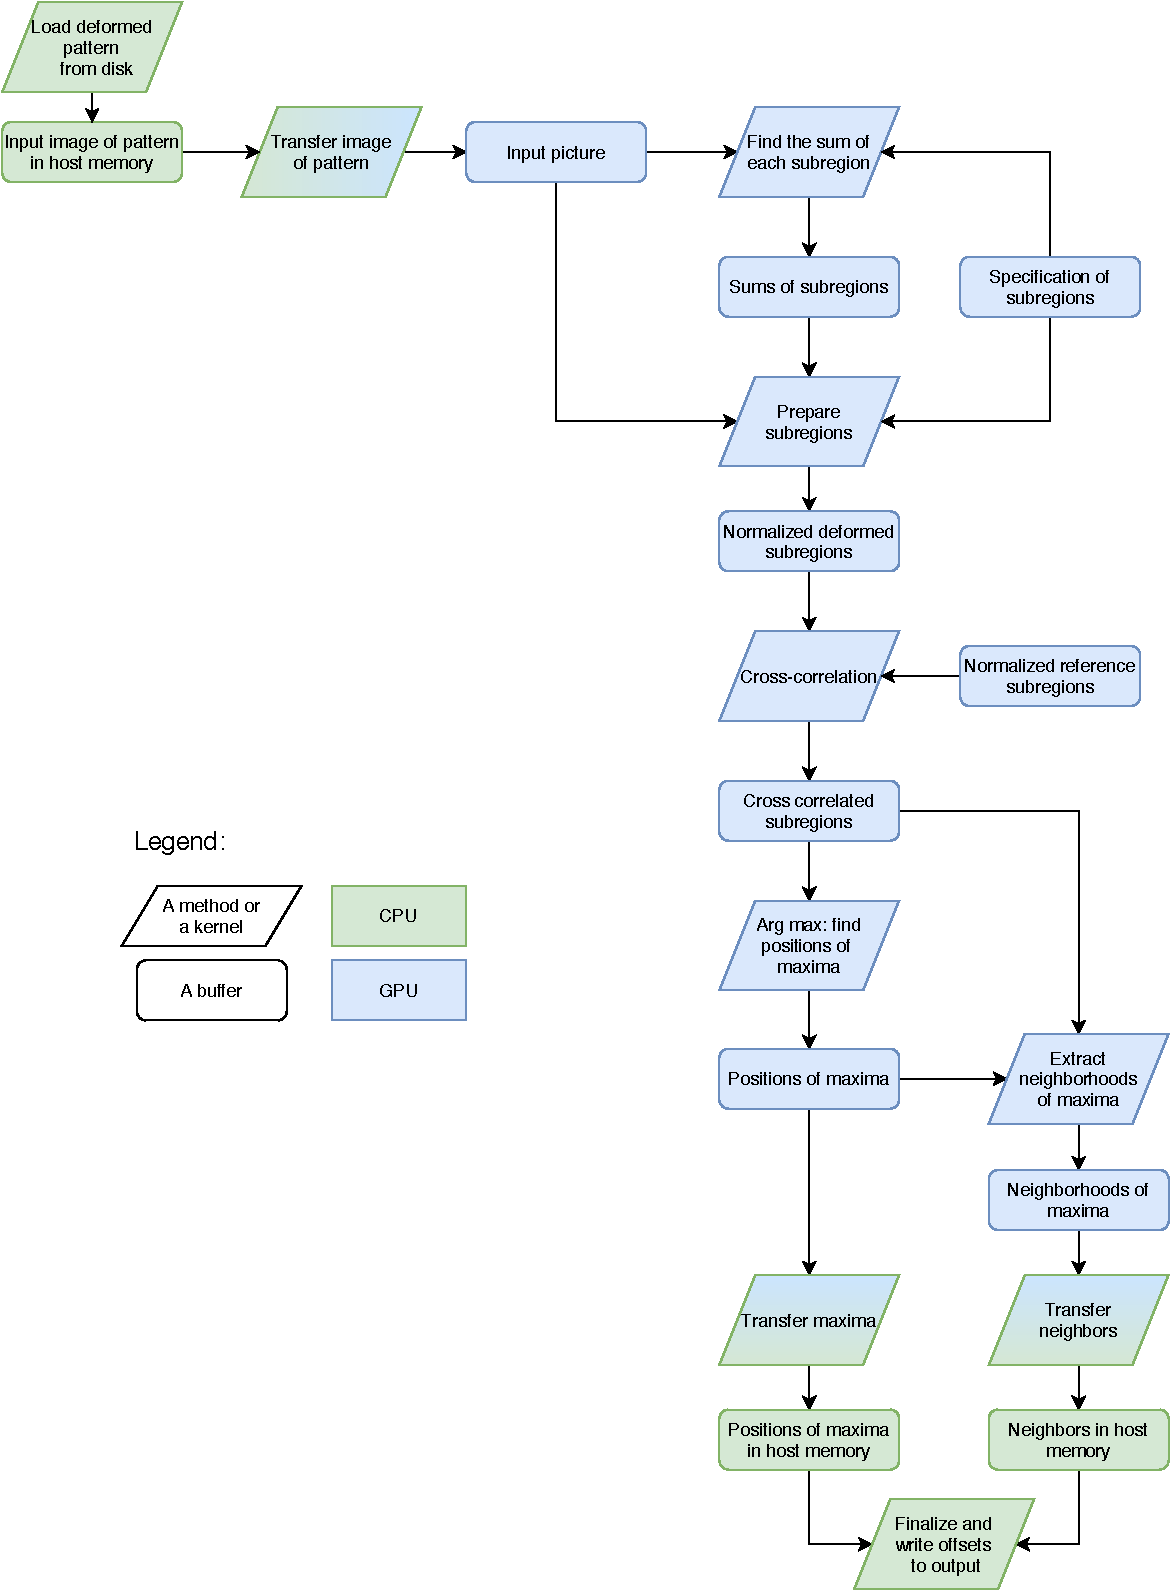
\includegraphics[width=\textwidth]{img/overview}
	\caption{Processing of one deformed pattern.}
	\label{overview}
\end{figure}

\Cref{overview} shows the data flow of the implementation and its decomposition into kernels. The processing starts with loading an image of a pattern from disk and its transfer to GPU. We transfer the whole pattern, as opposed to transferring only the subregions of interest.  Although we may end up copying data that the GPU never uses, this approach turned out to be better, because then we can utilize GPU when copying the subregions from the pattern. Moreover, we expect the regions to overlap in typical use case, so transferring the whole pattern copies less data.

The image is represented as an array of all the pixels in row--major order. Each pixel is an unsigned integer. 

Next, we need to prepare the data for cross--correlation --- copy the subregions from the image of deformed pattern and normalize them by subtracting the respective means. It is done in two kernels: \emph{sums} kernel and \emph{prepare} kernel. The sums kernel computes the sum of pixels of each subregion using parallel reduction. The prepare kernel extracts the subregions from the pattern, so that they are organized one after another in the output buffer: first, there all the pixels of the first subregion in row--major order, then all the pixels from the second and so on. Moreover, the kernel uses the sums from the first kernel to compute the mean for each region and subtracts it from each pixel of respective subregion.

The following part cross--correlates the normalized deformed subregions with reference ones. Since each deformed pattern is compared to the same reference, we pre-compute it (i.e., subtract the means from its subregions) and store it in a buffer on the GPU before loading the first deformed pattern.

Then, we analyze the result of the cross--correlation --- we find where is the maximum of each subregion using parallel reduction (\emph{arg max} kernel). The result is an array of coordinates of the maximum values (we are not interested in the values themselves). The next kernel then extracts a square shaped neighborhood of each maximum into one continuous buffer, so it can be transferred to the CPU memory together with the positions of the maxima.

The last part of the algorithm fits a continuous quadratic function to the neighborhood and then finds its maximum. We did not implement it for GPU, because it is not computationally demanding. It processes only a small neighborhood compared to the expected size of subregions. That also makes it cheap to transfer the maxima and neighborhoods from GPU to finish the computation on CPU and write the results to the output.

The decomposition into kernels is mostly determined by the need of global barriers. Both finding of sum and arg max use parallel reduction, which has to fully finish before any of its results are complete. The kernel that extracts the subregions from the pattern is necessary to simplify the cross--correlation and allow usage of third party libraries (see \cref{fft}, where the implementation of cross--correlation is explained).

To illustrate the data flow better and reason about it, \cref{params} summarizes parameters of the algorithm and \cref{buftypes} shows all buffers used on GPU with their sizes. The kernels that compute sums and normalize the subregions both work with $W_r \cdot H_r \cdot S$ items (i.e. all subregions). The cross--correlation has nearly four times as big output, which is then processed by the arg max kernel. After the maximum reduction, the buffers that are transferred to the CPU memory are quite small.

\begin{table}[]
	\begin{tabular}{@{}lll@{}}
		\toprule
		Buffer                          & Type         & Number of elements             \\ \midrule
		Input picture                   & uint16       & $W_p \cdot H_p$                \\
		Sums of subregions              & uint32       & $S$                            \\
		Positions of subregions         & uint32 pair  & $S$                            \\
		Normalized deformed subregions  & float/double & $W_r \cdot H_r \cdot S$        \\
		Normalized reference subregions & float/double & $W_r \cdot H_r \cdot S$        \\
		Cross--correlated subregions    & float/double & $(2W_r-1)\cdot(2H_r-1)\cdot S$ \\
		Positions of maxima             & uint32 pair  & $S$                            \\
		Neighborhoods of maxima         & float/double & $F^2 \cdot S $                 \\ \bottomrule
	\end{tabular}
	\caption{Summary of GPU buffers with their data types and size.}
	\label{buftypes}
\end{table}

The \cref{buftypes} also shows the data types stored in the buffers. The input image consists of unsigned 16 bit integers, so 4 byte unsigned integer is enough to hold the sums of its subregions of expected size. Once the means are subtracted, we use single or double floating point type --- when computing with 4 byte float, the implementation is substantially faster, however we are not sure whether it is precise enough, so we leave the choice as a parameter for our implementation.

\subsection{Task parallelization}

Since some parts of the algorithm are done on CPU and some on GPU (see color distinction in \cref{overview}), it is possible to parallelize them. There are 3 parts separated by data transfers between the main and the GPU memory: CPU first loads a pattern, GPU processes it, and then CPU does the finalization of results. It is desirable that we parallelize those tasks, so that GPU is fully utilized and never waits for the CPU.

\begin{figure}
	\centering
	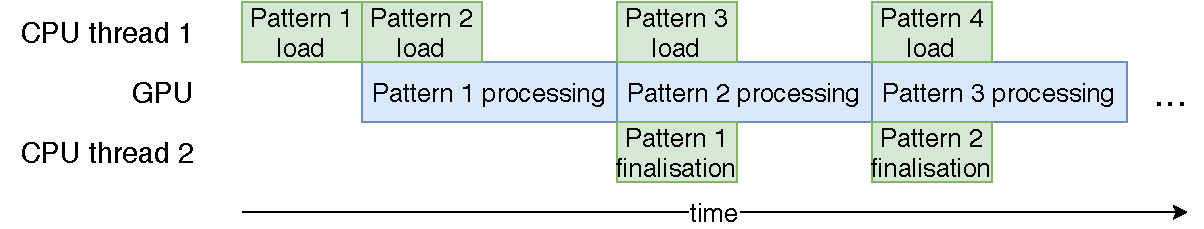
\includegraphics[width=\textwidth]{img/CPUGPUparal}
	\caption{Parallelization of GPU and CPU work.}
	\label{pipeline}
\end{figure}

\Cref{pipeline} shows how the work can be can be parallelized using a pipeline-like design. We use 2 worker CPU threads. While the GPU processes $i$-th pattern, one CPU thread already loads pattern $i+1$ and the second thread finalizes pattern $i-1$. The CPU work still takes much less time, so it is enough to start the load of pattern $i$ once processing of pattern $i-2$ finishes (and processing $i-1$ starts). That way, we do not need queues to pass work (like in the common pipeline pattern), we just need 2 buffers: one for writing the processed/prepared data and one for reading data to process. In the next iteration, we just swap the buffers.

We also partially take advantage of the fact that GPUs are able to run a kernel, copy data from and to memory at the same time. Actually, all transfers run in parallel with kernel execution. The host--device copy of input takes place right after the CPU loads the pattern from disk. Similarly, once the maxima and neighborhoods are prepared on the GPU, we start asynchronous transfer of the results and GPU starts computing the next pattern immediately. Unfortunately, this optimization does not affect performance much, since the copying between GPU and CPU memory takes only a marginal fraction of overall time.

In the following sections, we describe the implementation details of each individual kernel.

\section{Sum computation}
\label{sums}

Computation of sum is a textbook example of parallel reduction. In \cite{parallelReduction}, Justin Luitjens explains how to implement it on modern GPUs. Since it is very expensive to communicate between arbitrary threads during computation, the reduction is separated into two steps: first, we reduce the data within each block individually and only then we synchronize single value for each block.

The major difference for our case is that we compute a sum for each subregion, instead of computing a sum for the whole input data. The problem is that we cannot load values of two different subregions into one block. We solve this by assigning whole blocks to the subregions rather than just assigning threads to pixels. Let $B$ and $P$ denote one block size and total number of pixels in one subregion, respectively. Then we use a group of $S_1~=~\ceil{\frac{P}{B}}$ blocks for reduction of each subregion. Inside each block, we assign one thread per pixel in row-major order, so adjacent threads access adjacent data. It also means that the last block in each group is not fully utilized, because there is no more pixels in the subregion.

Once each thread loads its data, it is possible to reduce them fast within each block. We use warp--level shuffle instructions, which allows the threads in one warp to exchange data in registers. \Cref{warp_reduce} shows how it is possible to get sum of values in 8 threads. It can be expanded to size of warp, i.e. 32 threads. To reduce the whole block, we use the warp reduction in two steps:
\begin{enumerate}
	\item We perform the reduction within each warp and save the values into shared memory.
	\item One warp loads the values from the shared memory and reduces them using warp--level reduction again
\end{enumerate}
Maximum number of threads in one block is 1024 in CUDA and warp size is 32 so we get at most $1024/32 = 32$ values in the first step. That means one warp is enough to reduce them into one resulting value in the second step.

\begin{figure}
	\centering
	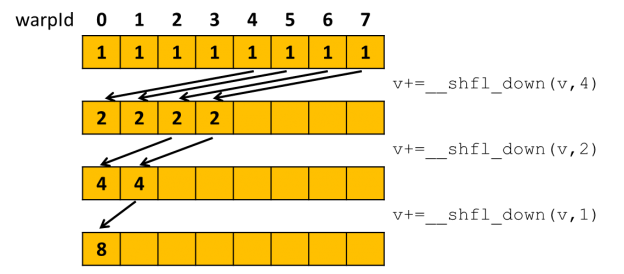
\includegraphics[width=0.7\textwidth]{img/warp_reduce}
	\caption{An example of warp--level reduction for 8 threads \cite{parallelReduction}. \emph{warpId} is a number of thread within its warp.}
	\label{warp_reduce}
\end{figure}

After reduction within each block, we need to update the resulting values in global memory, which requires more blocks working with the same value, possibly in parallel. On modern hardware, we solve such situations with atomic operations --- in our case of computing the sums it is \emph{atomic add}. The solution is feasible for us, since it is safe to assume that not many blocks access the same value. The typical size of one subregion is $100 \times 100$ which is the total of 10000 pixels. If we set the block size to 1024 (there is no reason not to use the maximal possible value --- no register or shared memory pressure), then only 10 blocks compute the sum of one subregion.

It is possible to further optimize the described technique by increasing the number of values each thread loads before the reduction begins. The problem is that half of the threads do (almost) nothing useful in the whole reduction: each of them only loads one value in the very beginning and immediately passes it to another thread (using shuffle instruction) which does the actual sum. So instead of loading only one value, each thread loads $N$ values and all the threads are utilized in the first part of the algorithm. It also means that we need $N$ times less blocks which may cause that for too high $N$, there will not be enough blocks to utilize the GPU. We measure the impact of the parameter in section ??.

\section{Prepare kernel}
Once the sums are computed, we need to subtract them from each pixel of respective subregion. We use the \emph{prepare} kernel to do that and to copy the subregions from the pattern so they are stored continuously in one buffer. If some subregions are overlapping, we copy some of the data twice, but then we subtract different means from them in general, so the result does not have any duplicities.

The kernel is fairly straightforward, we assign one thread to each pixel in each subregion. The threads compute the position of their pixel in the pattern using the buffer with the positions of the subregions, then compute mean using the sums buffer, subtract it and finally write the value to the output buffer.


\section{Arg max computation}
The cross--correlated data are further processed to find the position of maximum for each subregion by using parallel reduction. The computation is very similar to the sums reduction explained in \cref{sums} we use warp--level shuffle instructions and shared memory to reduce the values loaded to each block. The difference compared to sum reduction is that we need to find the maximum and its position at the same time. So throughout the algorithm, we operate on the pair of value and its position. Every time we compare two values and choose the higher one, we propagate its position as well.

Otherwise the reduction within one block is analogous to the sum reduction. In each step we shuffle down the current value and its position (that means two shuffles per one step). Then we compare the received and current value and save the greater one with its position for the next step. We need five these steps to reduce one warp, then each warp saves its result to the shared memory. Finally, one warp reduces the items in the shared memory to get the result of one block reduction.

In the sums reduction kernel, we used built-in atomic add to update the global memory with the result of block reduction. No such function exists for arg max, since we need to atomically compare two values and then update the position as well. There are several ways how do the update without the atomic operation.

\begin{description}
	\item[Launch second kernel] The first kernel does no synchronization between the blocks and each block just writes its reduced result to its reserved place in global memory. Then, we start second kernel which reduces the results of the first one. In the second kernel, all the values from one subregion are reduced by one block, so there is no synchronization needed anymore. 
	\item[One block reduces one whole subregion] We increase the number of values that each thread loads before the reduction, so only one block is needed to find the maximum of each subregion. Therefore, no synchronization across blocks is needed. Depending on the number of subregions, there is a possibility that this approach does not spawn enough blocks to fully utilize the GPU.
	\item[Atomic compare and swap (float data only)] We can use the atomic compare and swap (CAS) instruction to update the global memory atomically. There are not many blocks that would compete over the same piece of memory, so it is a viable solution. However, it can only be done when we compute the cross--correlation in single precision floating point type, since modern GPUs only support atomic CAS for 8 bytes. A double precision number is 8 bytes long itself, and we need to update the pair of value and its position.
\end{description}

The different approaches are compared in chapter 3.

\section{Extract neighbors kernel}

Once we compute the position of cross--correlation maximum for each subregion, we need to transfer the maxima and their neighborhoods from GPU to main memory so that the CPU can finalize and output the offsets. The maxima are already ready to transfer as a result of the arg max kernel, but we need to start another kernel to copy the neighborhoods from the cross--correlation into its own buffer, so we do not have to transfer the whole cross--correlation.

Recall that $F$ denotes the size of the square neighborhood. Given a maximum $[x_m, y_m]$, its neighborhood are the points $\{x_m - \frac{F-1}{2}, \cdots, x_m, \cdots, x_m + \frac{F-1}{2}\} \times \{y_m - \frac{F-1}{2}, \cdots, y_m, \cdots, y_m + \frac{F-1}{2}\}$ of cross--correlation. $F$ is always an odd number, so that the maximum is in the middle of the neighborhood. So the output buffer has size $F^2 \cdot S$, because each neighborhood has $F \cdot F$ points and there are $S$ subregions.

In the kernel, we assign one thread to each point of the neighborhood. Each thread computes the address of its point and copies it from the cross--correlation buffer to the neighborhoods buffer.

This kernel works with very small amount of data compared to other kernels, since $F$ is expected to be less than 10. Therefore the running time of this kernel is marginal and does not offer much space for improving overall running time.

\section{Offsets finalization}

When we have the positions of maxima and their neighborhoods lined up in two buffers, we transfer them to the CPU memory, since the finalization of the offsets takes place on the CPU. We compute the locations of maxima of the neighborhoods with subpixel accuracy as explained in \cref{subpixel-peak}. With the precomputed least squares matrix, the estimation of the quadratic function coefficients is a matter of one matrix--vector multiplication. Then, we compute the location of maximum of the quadratic function using two simple formulas. That gives us the location of the maximum relative to each neighborhood. In the final step, we combine the location of neighborhoods transfered from the GPU with the relative subpixel location of maxima within the neighborhoods and write out the resulting offset.
